\documentclass[tikz,border=2pt]{standalone}
\usepackage{amsmath}
\usepackage{pgfplots}
\pgfplotsset{compat=1.18}

\begin{document}
% f(x)=x^3/3-x: concave on the left of 0 (f''<0), convex on the right (f''>0); at the inflection
% point x=0 the tangent line crosses the graph.
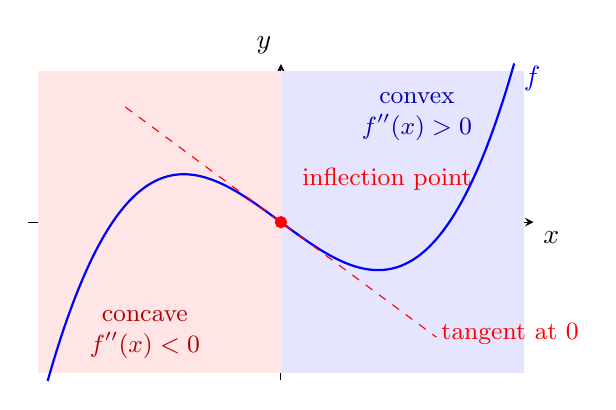
\begin{tikzpicture}
	\begin{axis}[
		axis lines=middle,
		xmin=-2.6, xmax=2.6,
		ymin=-2.2, ymax=2.2,
		xtick=\empty, ytick=\empty,
		xlabel={$x$}, ylabel={$y$},
		xlabel style={below right}, ylabel style={above left},
		samples=150, smooth, clip=false,
		width=8cm, height=5.6cm
		]
		\fill[red!10] (axis cs:-2.5,-2.1) rectangle (axis cs:0,2.1);
		\fill[blue!10] (axis cs:0,-2.1) rectangle (axis cs:2.5,2.1);
		\addplot[thick, blue, domain=-2.4:2.4] {x^3/3-x};
		\addplot[red, dashed, domain=-1.6:1.6] {-x};
		\addplot[only marks, mark=*, red] coordinates {(0,0)};
		\node[red, anchor=south west, font=\small] at (axis cs:0.12,0.3) {inflection point};
		\node[red!70!black, anchor=north, font=\small, align=center] at (axis cs:-1.4,-1.1) {concave\\ $f''(x)<0$};
		\node[blue!70!black, anchor=south, font=\small, align=center] at (axis cs:1.4,1.0) {convex\\ $f''(x)>0$};
		\node[red, anchor=west, font=\small] at (axis cs:1.55,-1.55) {tangent at $0$};
		\node[blue, anchor=west] at (axis cs:2.4,2.0) {$f$};
	\end{axis}
\end{tikzpicture}
\end{document}
